% Inbuilt themes in beamer
\documentclass{beamer}

% Theme choice:
\usetheme{Madrid}
\usepackage{setspace}
\usepackage{amssymb}
\usepackage{amsthm}
\usepackage{mathrsfs}
\usepackage{enumitem}
\usepackage{mathtools}
\usepackage{listings}
    \usepackage{color}                                            %%
    \usepackage{array}                                            %%
    \usepackage{longtable}                                        %%
    \usepackage{calc}                                             %%
    \usepackage{multirow}                                         %%
    \usepackage{hhline}                                           %%
    \usepackage{ifthen}                                           %%
    \usepackage{lscape}     
    \usepackage{amsmath}
       
\lstset{
%language=C,
frame=single, 
breaklines=true,
columns=fullflexible
}
\def\inputGnumericTable{}
\providecommand{\pr}[1]{\ensuremath{\Pr\left(#1\right)}}
\providecommand{\cbrak}[1]{\ensuremath{\left\{#1\right\}}}
\providecommand{\brak}[1]{\ensuremath{\left(#1\right)}}
\newcommand*{\permcomb}[4][0mu]{{{}^{#3}\mkern#1#2_{#4}}}
\newcommand*{\perm}[1][-3mu]{\permcomb[#1]{P}}
\newcommand*{\comb}[1][-1mu]{\permcomb[#1]{C}}
% Title page details: 
\title{Assignment 6 - Presentation} 
\author{CS21BTECH11024 - Varshini Jonnala}
\date{\today}

\begin{document}

% Title page frame
\begin{frame}
    \titlepage 
\end{frame}

% Outline frame
\begin{frame}{Outline}
    \tableofcontents
\end{frame}

\section{Abstract}
\begin{frame}{Abstract}
    \begin{itemize}
        \item This document contains the solution to Question 17 of Exercise-13.4 in Class 12 NCERT Book. 
    \end{itemize}
\end{frame}

% Lists frame
\section{Question}
\begin{frame}{Question}
Suppose that two cards are drawn at random from a deck of cards. Let $X$ be the
number of aces obtained. Then the value of $E(X)$ is
\end{frame}

% Blocks frame
\section{Solution}
\begin{frame}{Solution}
     Let the random variable $X \in \cbrak{0,1,2}$ denote the number of aces obtained when two cards are drawn at random from a deck of 52 cards. So, when two cards are drawn at random, the events are described as follows:

    \begin{table}[ht!]
        \centering
        \def\ifundefined#1{\expandafter\ifx\csname#1\endcsname\relax}
\ifundefined{inputGnumericTable}
	\def\gnumericTableEnd{\end{document}}

	\documentclass[12pt%
			  %,landscape%
                    ]{report}
       \usepackage[latin1]{inputenc}
       \usepackage{fullpage}
       \usepackage{color}
       \usepackage{array}
       \usepackage{longtable}
       \usepackage{calc}
       \usepackage{multirow}
       \usepackage{hhline}
       \usepackage{ifthen}
       \usepackage[misc]{ifsym}
	\begin{document}
\else
    \def\gnumericTableEnd{}
\fi
\providecommand{\gnumericmathit}[1]{#1} 
\providecommand{\gnumericPB}[1]%
{\let\gnumericTemp=\\#1\let\\=\gnumericTemp\hspace{0pt}}
 \ifundefined{gnumericTableWidthDefined}
        \newlength{\gnumericTableWidth}
        \newlength{\gnumericTableWidthComplete}
        \newlength{\gnumericMultiRowLength}
        \global\def\gnumericTableWidthDefined{}
 \fi
 \ifthenelse{\isundefined{\languageshorthands}}{}{\languageshorthands{english}}                                                      %%
\providecommand\gnumbox{\makebox[0pt]}                       %%
\setlength{\bigstrutjot}{\jot}
\setlength{\extrarowheight}{\doublerulesep}
\setlongtables

\setlength\gnumericTableWidth{%
	50pt+%
	170pt+%
0pt}
\def\gumericNumCols{4}
\setlength\gnumericTableWidthComplete{\gnumericTableWidth+%
         \tabcolsep*\gumericNumCols*2+\arrayrulewidth*\gumericNumCols}
\ifthenelse{\lengthtest{\gnumericTableWidthComplete > \linewidth}}%
         {\def\gnumericScale{1*\ratio{\linewidth-%
                        \tabcolsep*\gumericNumCols*2-%
                        \arrayrulewidth*\gumericNumCols}%
{\gnumericTableWidth}}}%
{\def\gnumericScale{1}}


\ifthenelse{\isundefined{\gnumericColA}}{\newlength{\gnumericColA}}{}\settowidth{\gnumericColA}{\begin{tabular}{@{}p{50pt*\gnumericScale}@{}}x\end{tabular}}
\ifthenelse{\isundefined{\gnumericColB}}{\newlength{\gnumericColB}}{}\settowidth{\gnumericColB}{\begin{tabular}{@{}p{170pt*\gnumericScale}@{}}x\end{tabular}}

	\begin{center}
\begin{tabular}[c]{%
	b{\gnumericColA}%
	b{\gnumericColB}%
	}

	\hhline{|-|-~}
	 \multicolumn{1}{|p{\gnumericColA}|}%
	{\gnumericPB{\centering}\gnumbox{\textbf{Event}}}
	&\multicolumn{1}{p{\gnumericColB}|}%
	{\gnumericPB{\centering}\gnumbox{\textbf{Description}}}
\\
    \hhline{|--|~}
	 \multicolumn{1}{|p{\gnumericColA}|}%
	{\gnumericPB{\centering}\gnumbox{$X=0$}}
	&\multicolumn{1}{p{\gnumericColB}|}%
	{\gnumericPB{\centering}\gnumbox{Hanif losing the game}}
\\
    \hhline{|--|~}
	 \multicolumn{1}{|p{\gnumericColA}|}%
	{\gnumericPB{\centering}\gnumbox{$X=1$}}
	&\multicolumn{1}{p{\gnumericColB}|}%
	{\gnumericPB{\centering}\gnumbox{Hanif winning the game}}
\\
\hhline{|-|-|~}
\end{tabular}
	\end{center}
	
\ifthenelse{\isundefined{\languageshorthands}}{}{\languageshorthands{\languagename}}
\gnumericTableEnd

    	\caption{Description of Events}
    	\label{Tables:Table}
    \end{table}
\end{frame}    

    \begin{align}
        \pr{X = 0} = \frac{\comb{4}{0} \comb{48}{2}}{\comb{52}{2}} = \frac{1128}{1326}\\
         \pr{X = 1} = \frac{\comb{4}{1} \comb{48}{1}}{\comb{52}{2}} = \frac{192}{1326}\\
          \pr{X = 2} = \frac{\comb{4}{2} \comb{48}{0}}{\comb{52}{2}} = \frac{6}{1326}
    \end{align}
    The probability distribution is as follows:
    \begin{align}
    E\brak{X} &= \sum_{i = 1}^{n}x_i \times \pr{x_i}\\
    &= 0 \times \frac{1128}{1328} + 1 \times \frac{192}{1328} + 2\times \frac{6}{1326}\\
    &= \frac{204}{1326}\\
    &= \fbox{$\frac{2}{13}$}
    \end{align}
    
\section{Graph}
\begin{frame}{PMF Graph}
The PMF graph is:
    \begin{figure}[!ht]
		\centering
		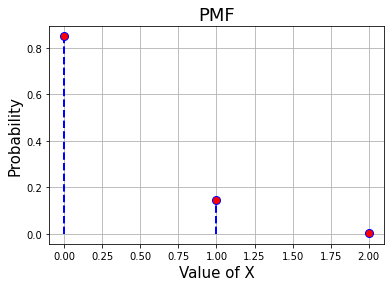
\includegraphics[width=\textwidth,height=5.5cm,keepaspectratio]{pmf.png}
		\caption{Probability Mass Function}
		\label{fig1}
	\end{figure}
\end{frame}
\end{document}
